\documentclass[11pt]{article}

\usepackage[utf8]{inputenc}
\usepackage[french]{babel}

% TODO 1. Géométrie
\usepackage[a4paper,margin=1in,portrait]{geometry}

\usepackage[table]{xcolor}
\definecolor{lightgray}{gray}{0.85}
\definecolor{verylightgray}{gray}{0.95}
\let\oldtabular\tabular
\let\endoldtabular\endtabular
\renewenvironment{tabular}{\small\rowcolors{1}{lightgray}{verylightgray}\oldtabular}{\endoldtabular}

% Pour le bas de page
\newcommand{\mysmallgray}[1]{\scriptsize\color{gray}#1}

\usepackage{comment}

% Pour le strikethrough
%\usepackage{ulem}
%\sout{text}
\usepackage{amssymb}

%\usepackage{multicol}
%\setlength{\columnsep}{0.5cm}
%\usepackage{wrapfig}

\usepackage{textcomp}
% to use \textcopyleft

\usepackage{graphicx}
\graphicspath{{./yed/}{./images/}}

% TODO 2. Remplir les champs
\newcommand{\mytitle}{Risus MEGA}
\newcommand{\myauthor}{Olivier Rey}
\newcommand{\mysubject}{Jeu de rôles}
\newcommand{\mykeywords}{JDR,TTRPG,RPG,AideDeJeu,orey,méga,MEGA,messagers-galactiques}
\newcommand{\myversion}{1.1}
\newcommand{\mycolor}{violet}

% PDF
\usepackage{hyperref}
\hypersetup{
  a4paper=true,
  pdftitle={\mytitle},
  pdfauthor={\myauthor},
  colorlinks=true,
  linkcolor=blue,
  urlcolor=blue,
  pdfsubject={\mysubject},
  pdfkeywords ={\mykeywords},
  pdfstartview={FitH},
  bookmarksopen={false},
  bookmarksnumbered={true}
}

% TODO 3. Adapter le titre
\usepackage{fancyhdr}
\pagestyle{fancy}
\fancyhead[L]{}
\fancyhead[C]{{\color{\mycolor}\textbf{{\Huge R}{\LARGE ISUS - }{\Huge R}{\LARGE ÈGLES POUR }{\Huge M}{\LARGE ÉGA}}}}
\fancyhead[R]{}

\fancyfoot[L]{\mysmallgray{Version \myversion}}
\fancyfoot[C]{\mysmallgray{\today}}
\fancyfoot[R]{\mysmallgray{Copyleft \href{https://github.com/orey/jdr-risus}{Olivier Rey}}}
\renewcommand{\headrulewidth}{0.4pt}
\renewcommand{\footrulewidth}{0.4pt}

% Enlève l'indentation pour tout le documnt (équivalent de \noindent sur toutes les lignes)
%\setlength\parindent{0pt}

% Sections avec points après les numéros
\usepackage{titlesec}
\titlelabel{\thetitle.\quad}
\titleformat*{\section}{\color{\mycolor}\bfseries\Large}
\titleformat*{\subsection}{\color{\mycolor}\bfseries\large}
\usepackage[dotinlabels]{titletoc}

%\AtBeginDocument{
%  \addtocontents{toc}{\footnotesize}
%  \addtocontents{lof}{\footnotesize}
%}

% Mes macros

\begin{comment}
\newcommand{\mysection}[1]{
\vspace{0.2cm}
\noindent{\color{\mycolor}\large\textbf{#1}}
}

\newcommand{\mysubsection}[1]{
\vspace{0.1cm}
\noindent{\textit{\textbf{#1}}}
}
\end{comment}

%=======================================DOC
\begin{document}

%=============== Title page

\pagestyle{empty}

\begin{center}

\includegraphics[scale=0.30]{logo-risus}

\vspace{1.0cm}


\includegraphics[scale=1.0]{logo-mega-red}

\vfill

\begin{tabular}{ll}
Méga 1 (1984)       & \href{https://archive.org/details/jeux-et-strategie-hs-1}{Méga 1}, l'origine \\
Méga 2 (1986)       & L'indispensable \href{https://archive.org/details/jeux-et-strategie-hs-2}{Méga 2} \\
Méga 3 (1992)       & Ne peut être trouvé qu'en occasion, voir la fiche \href{https://www.legrog.org/jeux/mega/mega-3/mega-iii-fr-47583}{Grog} \\
Méga 4 (2012)       & Superbes encyclopédie et scenarii sur \href{https://www.messagers-galactiques.com}{messagers-galactiques.com} \\
Méga 5 (2018)       & La \href{https://www.legrog.org/jeux/mega/mega-5e-paradigme/mega-5e-paradigme-fr}{fiche} du Grog \\
Risus EN            & \href{https://www.drivethrurpg.com/product/170294/Risus-The-Anything-RPG}{Risus the RPG} \copyright\ Big Dice Games \\
Risus FR            & \href{https://github.com/orey/jdr-risus/blob/main/risus/risus-fr.pdf}{Risus, traduction de Tristan Lhomme} \\
Sites américains    & Nouveau site : \href{https://www.risusrpg.com}{risusrpg.com} \\
                    & Ancien site : \href{https://www.risusiverse.com/}{risuiverse} \\
Ressources Risus FR & \href{https://rouboudou.itch.io/risus}{rouboudou.itch.io/risus} \\
Copyleft            & Version \myversion\ -- \textcopyleft\ \href{https://rouboudou.itch.io}{Olivier Rey} 2022 \\
\end{tabular}
\end{center}

\vspace{0.2cm}

%Note : ce supplément utilise principalement des graphiques pour proposer des règles simples et visuelles.

\tableofcontents

%=============== Fin title page
\newpage
\pagestyle{fancy}

%======= mysection
% TODO Création du personnage
\section{Création du personnage}

Comme dans le jeu classique, tous les joueurs démarrent avec 10D de Création (10D$\Subset$) à répartir. Le personnage Méga dans Risus possède 4 types de clichés :

\begin{center}
\begin{tabular}{cccc}
\textbf{Cliché} & \textbf{Min} & \textbf{Max} & \textbf{Coût en D de création}\\
Cliché Méga	& 3D & 3D & 5D$\Subset$ $\rightarrow$ 3D de Cliché\\
Affinité Méga (option) & 0D & 3D & 1D$\Subset$ $\rightarrow$ 1D de Cliché\\
Pouvoirs psy (option) & 0D & 2D & 2D$\Subset$ $\rightarrow$ 1D de Cliché\\
Autres Clichés & 0D & 3D & 1D$\Subset$ $\rightarrow$ 1D de Cliché\\
\end{tabular}
\end{center}

\subsection{Le Cliché Méga}

Les Mégas possèdent deux talents, deux pouvoirs psychiques très importants dans les aventures : le Transit, et le Transfert (voir plus loin). Si l'on en croît les règles de Risus, pour avoir deux pouvoirs de ce type à 3D chacun, il faudrait que les joueurs investissent 6D (le coût d'un dé de pouvoir ou de magie est de 2D de création).

Nous proposons donc, afin pour un personnage  Méga de commencer avec 3D dans le \og Cliché Méga \fg, d'investir 5D pour pouvoir faire les \og trucs des Mégas \fg{}, à commencer par le Transit et le Transfert, mais pas seulement (les Mégas sont supposés avoir un certain entraînement).

\begin{center}
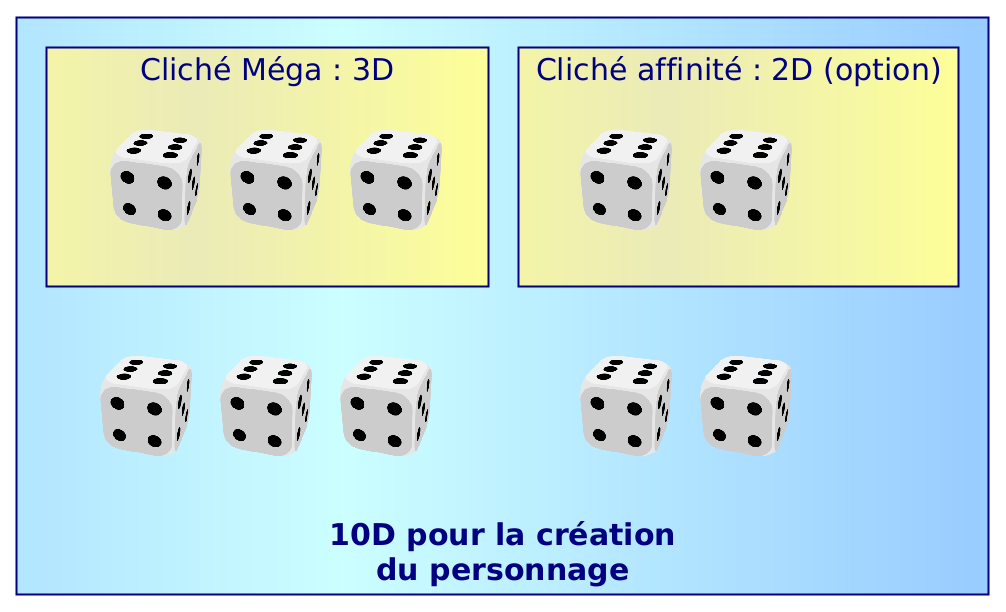
\includegraphics[scale=0.34]{01-creation-perso}
\end{center}

Exemple de Clichés Méga :
\begin{itemize}
\item Terrien Méga des montagnes,
\item Méga parisien impressionné par la grandeur de l'univers et réalisant que la Terre est en banlieue,
\item Méga vétéran kiffant les mondes parallèles,
\item Méga intello qui veut tout comprendre,
\item Jeune Méga hystérique de jouer avec ses pouvoirs,
\item Méga prudent et travailleur, ambitieux et ne voulant pas rester sur le terrain trop longtemps,
\item Méga qui a la trouille de se retrouver sur la Bételgeuse d'un monde parallèle,
\item Ancien de la FRAG ayant découvert ses pouvoirs Méga sur le tard,
\item Etc.. 
\end{itemize}

Le Cliché Méga des débutants est limité à 3D. Il peut progresser selon les règles de Risus.

\newpage
\subsection{L'affinité Méga}

Optionnellement, le Méga peut choisir une affinité (3D ou moins) ou lancer 2D et consulter le diagramme ci-dessous. L'affinité est aussi source de Clichés.

\begin{center}
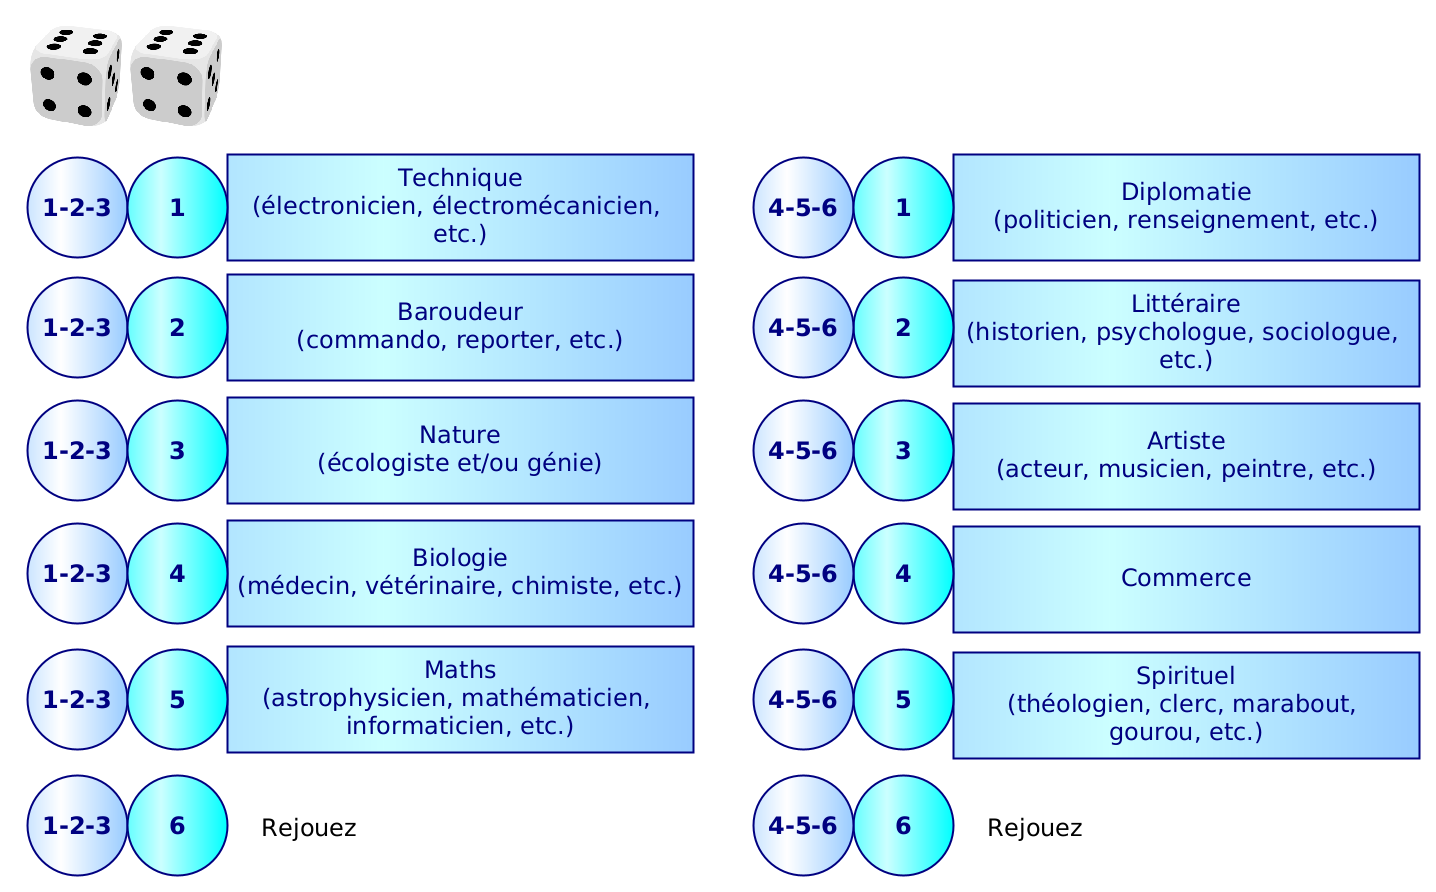
\includegraphics[scale=0.31]{02-affinite}
\end{center}

Le MJ et/ou les joueurs peuvent créer des affinités Mégas ne figurant pas dans cette liste. L'affinité est un genre de profil de personnages reconnu par la Guilde des Mégas.

\newpage
\subsection{Les pouvoirs psy}

Les Mégas possèdent déjà deux pouvoirs exceptionnels qui les rendent uniques au sein des univers : le Transit et le Transfert (couverts par le Cliché Méga, voir plus loin).

En supplément, le MJ peut autoriser les Mégas à disposer d'un autre pouvoir psy, soit choisi, soit tiré au sort dans la table ci-dessous. Le coût du pouvoir psy est de 2D$\Subset$ pour 1D de Cliché.

\begin{center}
\begin{tabular}{c l}

\includegraphics[scale=0.08]{dice.png} & \textbf{Pouvoir psy}\\
1 & Emprunte astrale \\
2 & Télékinésie \\
3 & Télépathie \\
4 & Lévitation \\
5 & Corps éthéral \\
6 & Rejouez \\
\end{tabular}
\end{center}

\begin{center}
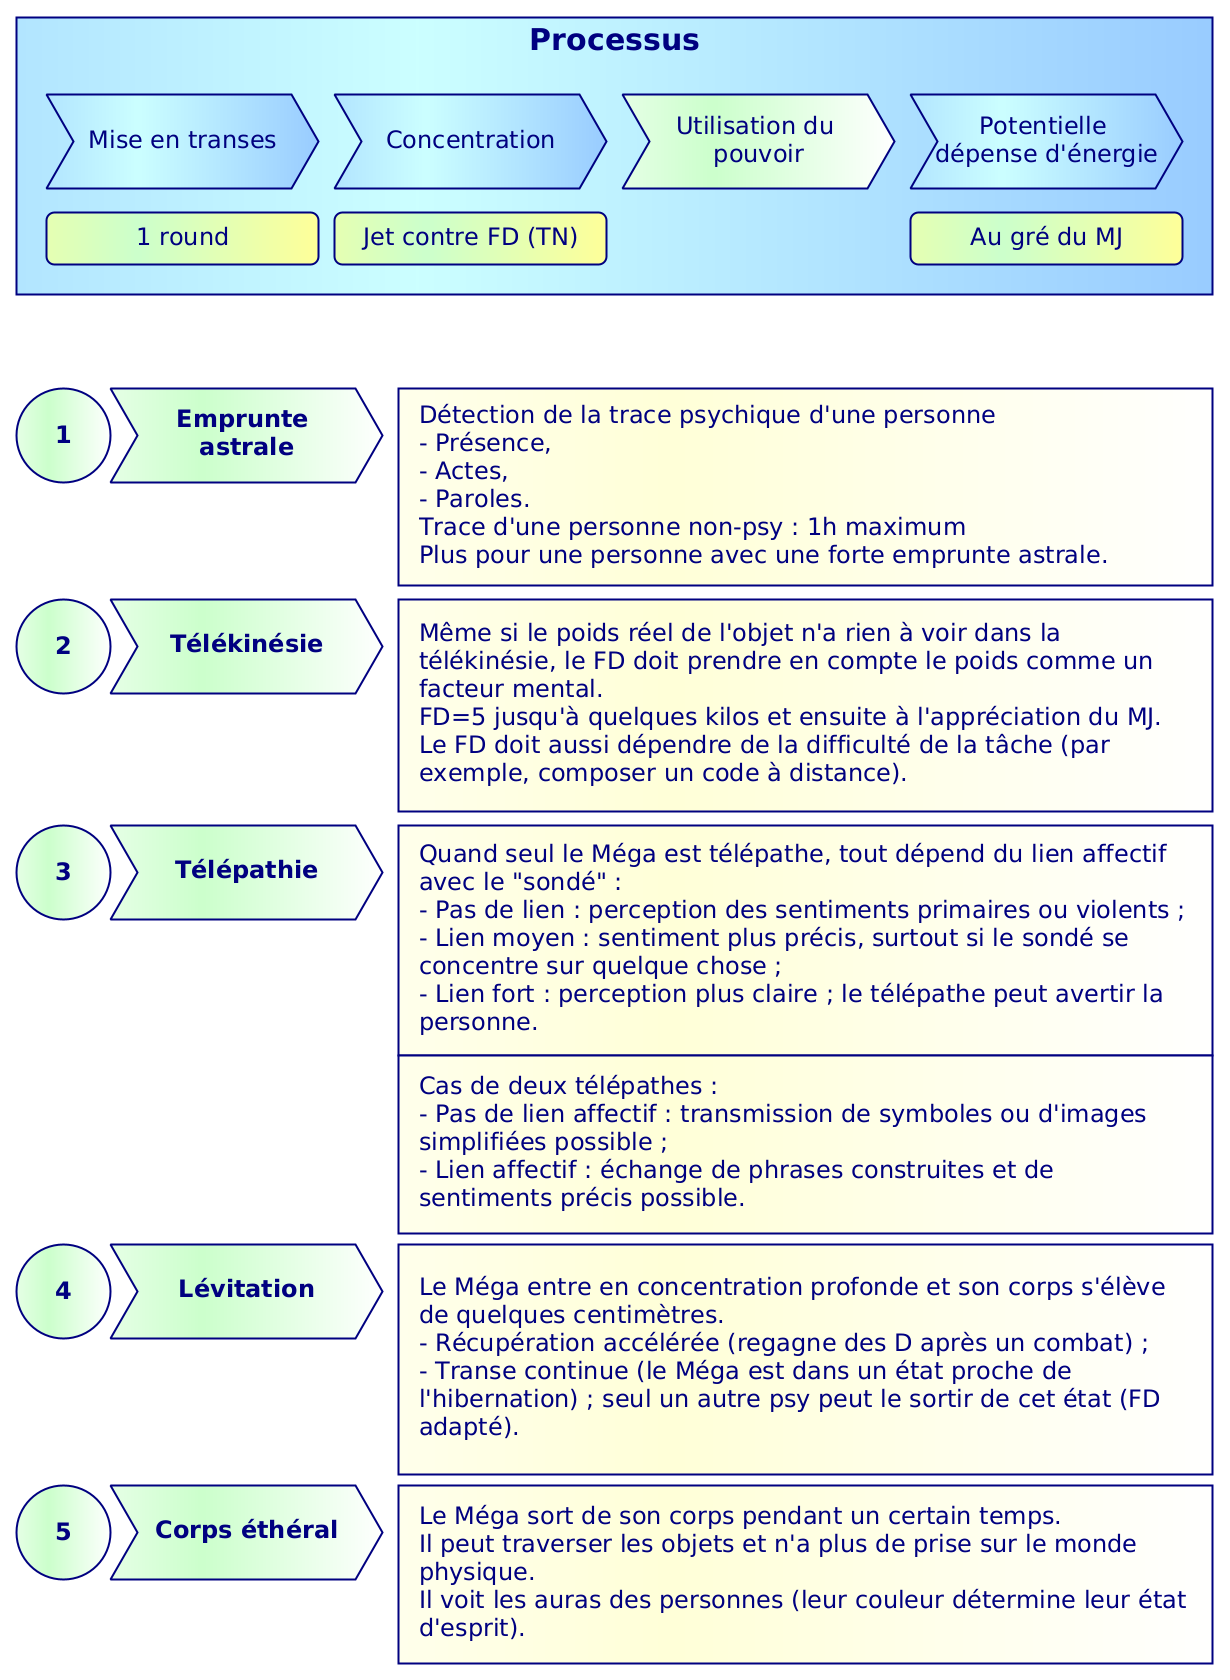
\includegraphics[scale=0.28]{03-pouvoirs-psy}
\end{center}

\newpage
%=================================Nouvelle page
%TODO Le Transit
\section{Le Transit}

\subsection{Règles du Transit}

Le Transit est la faculté de se téléporter au moyen d'un tétraèdre, soit dans le même univers, soit dans un univers parallèle.

Le processus est expliqué dans la figure ci-dessous.

\begin{center}
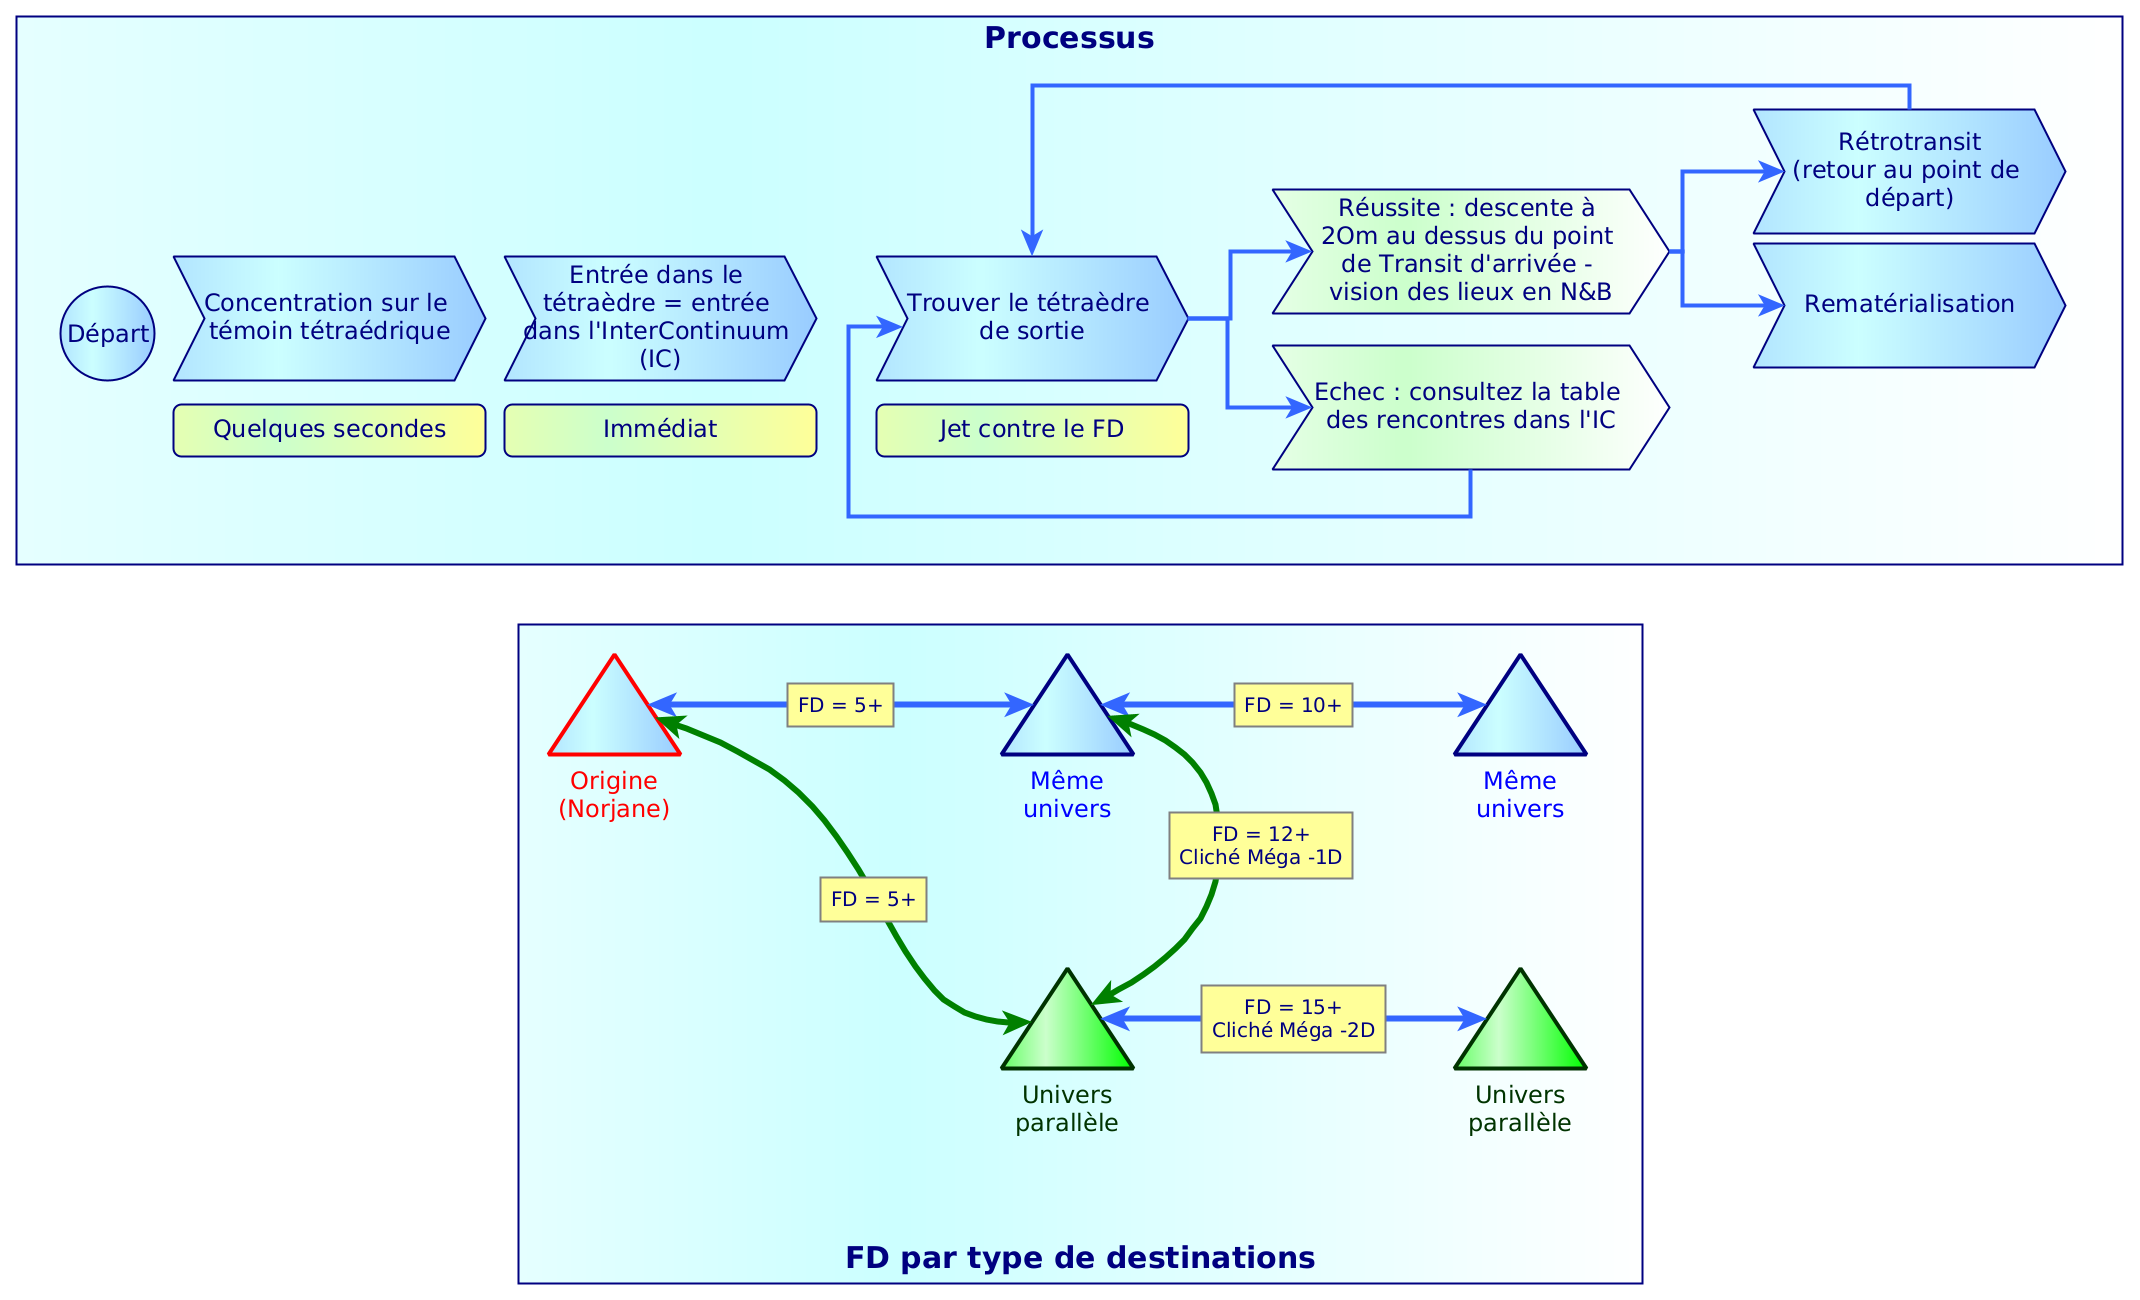
\includegraphics[scale=0.21]{04-transit}
\end{center}

\subsection{Échec du transit}

En cas d'échec du Transit, le PJ est bloqué dans l'Inter-Continuum (IC). Le joueur doit lancer 1D pour déterminer l'issue de l'échec (potentielle rencontre avec une créature de l'IC).

\begin{center}
\begin{tabular}{c l c}

\includegraphics[scale=0.08]{dice.png}+
\includegraphics[scale=0.08]{dice.png} & \textbf{Nature de l'échec} & \textbf{Lien}\\
2-7 & Transit raté                     & \hyperref[rate]{Table} des transits ratés \\
8   & Changeur                         & \hyperref[ic]{Table} des rencontres dans l'IC \\
9   & Fleurs de folie                  & \hyperref[ic]{Table} des rencontres dans l'IC \\
10  & Sirènes                          & \hyperref[ic]{Table} des rencontres dans l'IC \\
11  & Vampire                          & \hyperref[ic]{Table} des rencontres dans l'IC \\
12  & Guetteur ou autre entité de l'IC & \hyperref[ic]{Table} des rencontres dans l'IC \\
\end{tabular}
\end{center}

En cas d'échec, tout peut arriver, au gré du MJ. Si un PJ a créé un ou des points de transit, il a 50\% de chances d'aboutir sur un d'entre eux (tirer point après point). Sinon, le MJ peut consulter la table des transits ratés (en annexe).

\subsection{Transiter avec un autre être vivant}

Il est possible de transiter avec un autre être vivant, pourvu que l'on reste en contact avec lui. Le MJ peut ajouter un FD supplémentaire au FD du dessus (2+).

\subsection{Créer un point de Transit}

Le tétraèdre doit être constitué d'une matière dense et homogène. En plus du tétraèdre du point de Transit, le Méga doit avoir des petits tétraèdres témoin en contact avec l futur point de transit. 

Le MJ détermine la résistance du point de Transit en lançant 8D+.

Par exemple, supposons que la résistance du tétraèdre soit de 27. Le Méga doit accumuler plus de 27 points en faisant des jets contre un FD de 11 et en suivant le processus ci-dessous.


\begin{center}
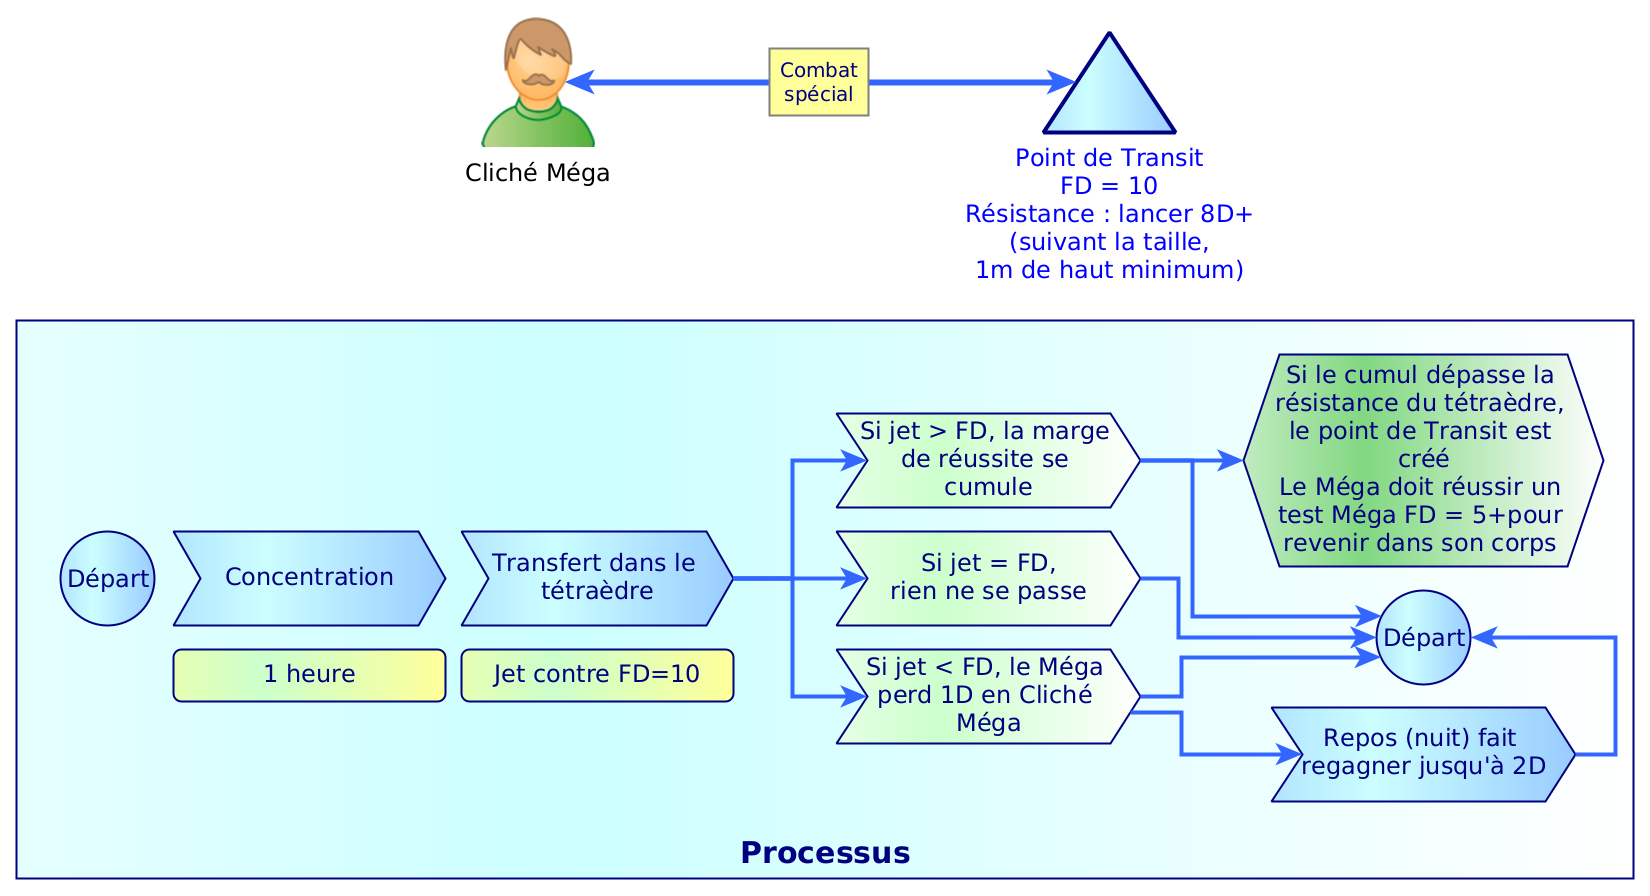
\includegraphics[scale=0.28]{05-point-transit}
\end{center}



\newpage
%=================================Nouvelle page
%TODO Le Transfert
\section{Le Transfert}

\subsection{Règles du Transfert}

Le Transfert est la capacité de se transférer dans le corps d'un autre être vivant. C'est un combat mental.

En cas de Transfert réussi, le corps du Méga tombe en catalepsie jusqu'à ce que le Méga le réintègre.

La figure ci-dessous explique le processus du Transfert.

\begin{center}
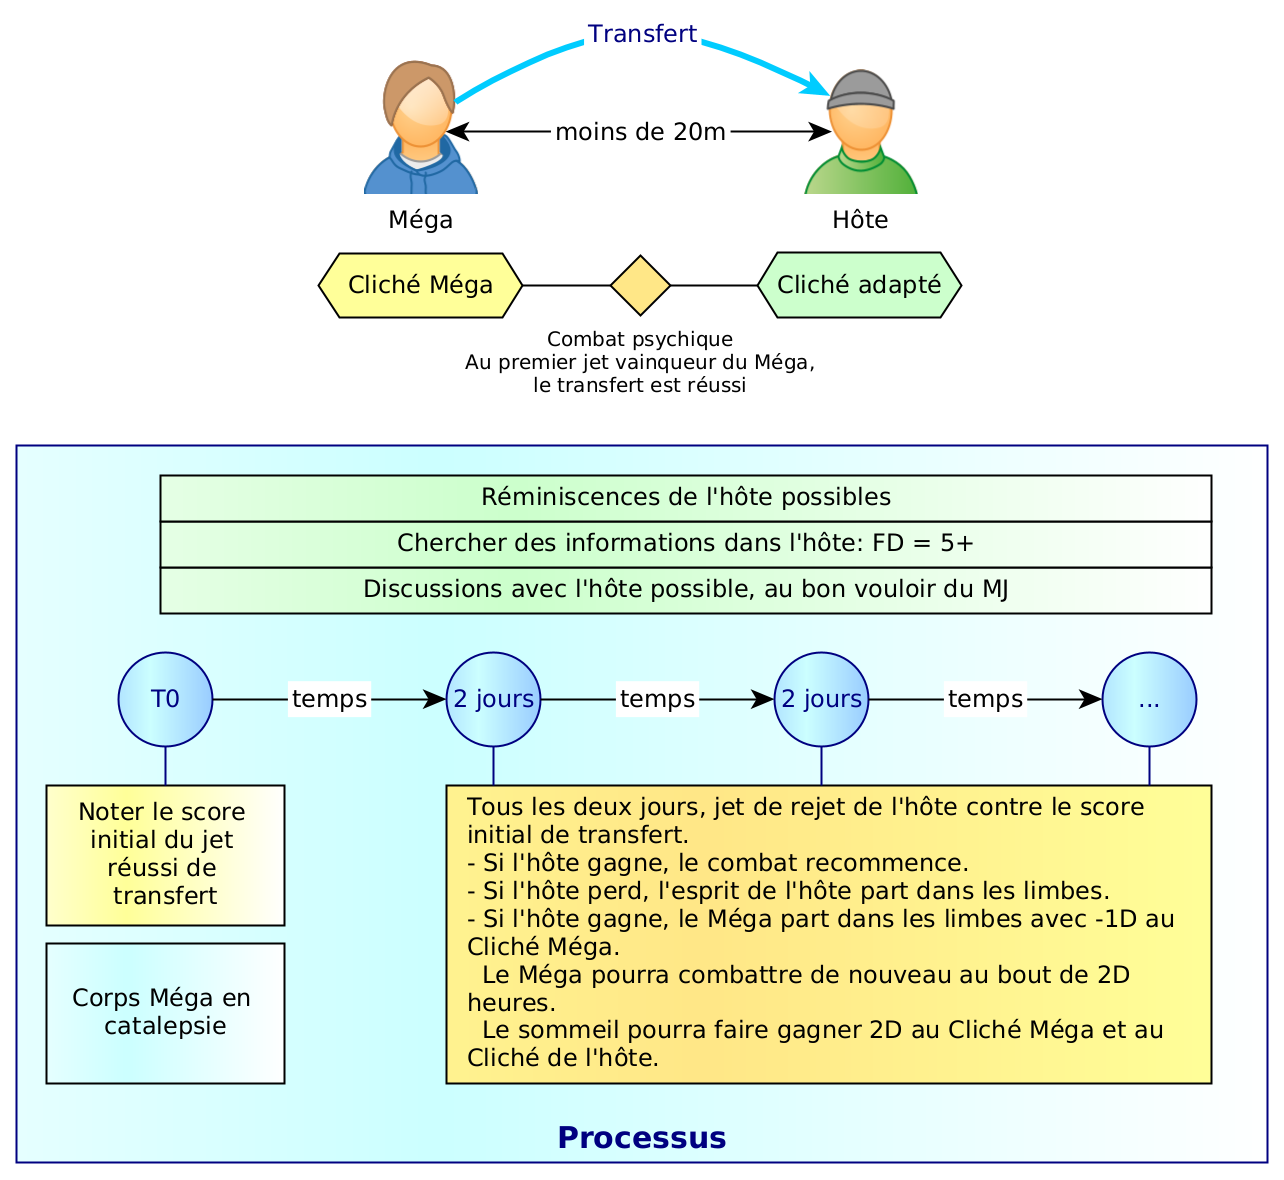
\includegraphics[scale=.35]{06-transfert}
\end{center}

\subsection{Transfert depuis un corps déjà transféré}

Un transfert depuis un corps transféré est un combat contre la somme des Clichés des hôtes :
\begin{itemize}
\item L'hôte de départ,
\item L'hôte d'arrivée.
\end{itemize}

\subsection{Retro-transfert}

Le Méga peut regagner son corps sans effort s'il se trouve à moins de 20 mètres de ce dernier. L'être vivant ayant subi le Transfert ne se souviendra de presque rien (vagues impressions, images, au bon vouloir du MJ).

\section{Annexes}

\subsection{Table des Transits ratés}
\label{rate}

\begin{center}
\begin{tabular}{c p{5.5cm} c p{5.5cm}}

\includegraphics[scale=0.08]{dice.png}
\includegraphics[scale=0.08]{dice.png} & \textbf{Destination} &

\includegraphics[scale=0.08]{dice.png}
\includegraphics[scale=0.08]{dice.png} & \textbf{Destination} \\
11 & Dans un univers à l'air empli d'un hallucinogène. Au bout d'1D heures, le Méga voit et entend des choses &
41 & Sous la calotte glaciaire \\
12 & Au sommet d'un piton rocheux &
42 & Sous les débris d'une avalanche \\
13 & Au cœur d'un désert aride &
43 & Sous les ruines d'une ancienne cité \\
14 & En zone radioactive ou contaminée par un virus &
44 & Sous des scories volcaniques \\
15 & Dans une zone où tout ce qui est comestible est empoisonné &
45 & Dans une décharge publique \\
16 & Chez des humanoïdes beaux et accueillants vouant un culte aux Mégas &
46 & Chez des extraterrestres NT6 effrayants mais très pacifiques, très intelligents et inconnus de l'AG \\
21 & Au fond d'un lac de montagne &
51 & Dans un vaisseau spatial extraterrestre \\
22 & Dans le lit d'un fleuve ou d'une rivière &
52 & Dans un astéroïde-prison \\
23 & Dans un marécage putride &
53 & Dans un zoo galactique \\
24 & Dans une mer chaude près d'une île déserte &
54 & Au milieu d'un terrain miné avec un écriteau "Interdit aux Mégas" \\
25 & Dans une mer froide voire glaciale &
55 & Sur une place du marché médiévale \\
26 & Dans la piscine d'une célébrité (par ex. Esther Lindon) &
56 & Au sommet d'un arbre-monde peuplé d'animaux pacifiques et intelligents\\
31 & Dans une énorme caverne &
61 & Dans une base Méga abandonnée depuis des siècles \\
32 & Dans un réseau de catacombes &
62 & Dans une base Méga abandonnée depuis quelques temps\\
33 & Dans un vaste abri anti-atomique &
63 & Sur une planète alien qui considère les Mégas comme des êtres répugnants \\
34 & Dans une ancienne mine abandonnée &
64 & dans une base secrète de renégats\\
35 & Dans un réseau de métro &
65 & Dans la base d'une Guilde inconnue\\
36 & Dans la cachette d'un fabuleux trésor &
66 & Sur l'une des "cinq lointaines" (base de vieux Mégas à la retraite) \\
\end{tabular}
\end{center}

\subsection{Table des rencontres dans l'InterContinuum (IC)}
\label{ic}

Les rencontres dans l'IC ont les caractéristiques suivantes.

\begin{center}
\begin{tabular}{c p{13.0cm}}
\textbf{Rencontre} & \textbf{Détails} \\
Changeur & Le changeur prend l'apparence du PJ avec quelques changements. Il discute avec le PJ. Si la discussion se passe mal, le PJ a quelque chose de changé. \\
Fleurs de folie & Jouent avec les pensées et les peurs du Méga en les matérialisant. Peuvent aller jusqu'à créer un univers de poche. \\
Sirènes & Attirent le Méga dans un paradis adapté à la personne. Test Cliché Méga pour résister avec un FD qui augmente progressivement (+1) en cas d'échec \\
Vampire & S'interpose et bloque l'accès au tétraèdre de sortie en obligeant à passer par un autre point de Transit ou à revenir en arrière. Combat mental avec le vampire 2D+ pour sortir \\
\end{tabular}
\end{center}

Voir l'\href{https://www.messagers-galactiques.com}{encyclopédie du messager galactique} pour plus de détails.

\end{document}
